\FloatBarrier
\section{Análise da Ferramenta Gemini Pro}
\label{s.ferramentaB}

A ferramenta Gemini Pro foi escolhida por sua capacidade de operar, entender e combinar diferentes tipos de informação, incluindo texto, imagem e vídeo \cite{sundarpichai_2023}. Mais especificamente, para os testes, foi utilizado o Gemini 2.5 Pro, que é capaz de raciocinar nativamente por meio de seus pensamentos antes de responder, o que aumenta a performance e a precisão \cite{koraykavukcuoglu_2025}. Para a geração de imagens, era integrado o modelo especializado Imagen 4, e para vídeos havia o Veo 3 \cite{woodward_2025}. 

Para a geração e edição de imagens, era possível anexar diversos arquivos, enquanto para a criação do vídeo só era permitido o anexo de uma imagem. Além disso, era oferecida a possibilidade de re-gerar as figuras com um limite alto, porém os vídeos tinham um limite diário de três gerações e não podiam ser refeitos sem escrever novamente o prompt.

Durante a análise, o objetivo variou de acordo com o sucesso dos testes e as necessidades do projeto. No total, foi tentado criar animações do personagem Pablo andando, pulando, abrindo a porta e de diferentes portas fechando.

%%% pablo, pablo lateral de alguma IA, ver tudo que pegou de fora
\begin{figure}[htbp]
    \centering
    \caption{\small Artefatos usados para referência no Gemini Pro}
    \label{fig:geminiProArtefatos}
    \begin{subfigure}{0.23\linewidth}
        
\includegraphics[width=0.7\linewidth]{figs/sprites/Pablo.PNG}
        \caption{\small Sprite do personagem Pablo em front view}
        \label{fig:geminiProPablo}
    \end{subfigure}
    \begin{subfigure}{0.22 \linewidth}
        \centering
        
\includegraphics[width=1\linewidth]{figs/chatGPT/visao_lateral/res1.png}
        \caption{\small Sprite do personagem Pablo em side view gerado pelo ChatGPT}
        \label{fig:geminiProPabloChatGPTSide}
    \end{subfigure}
    \begin{subfigure}{0.23\linewidth}
        \centering
        
\includegraphics[width=1\linewidth]{figs/pixelLab/dia2/fix_init_1.PNG}
        \caption{\small Sprite do personagem Pablo em side view gerado pelo Pixel Lab}
        \label{fig:geminiProPabloPixelLab}
    \end{subfigure}
    \begin{subfigure}{0.23\linewidth}
        
\includegraphics[width=1\linewidth]{figs/sprites/Pablo_sideView.png}
        \caption{\small Sprite do personagem Pablo em side view gerado pelo Gemini Pro e editado no Pixel Lab}
        \label{fig:geminiProPabloPixelLabSide}
    \end{subfigure}
    \begin{subfigure}{0.23\linewidth}
        \centering
        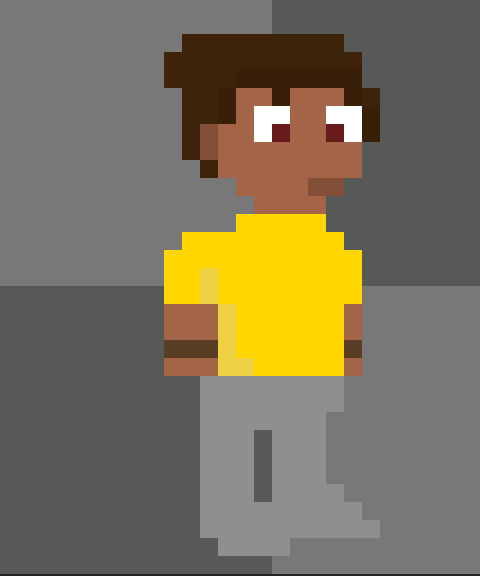
\includegraphics[width=1\linewidth]{figs/pixelLab/dia2/fix_teste_3.PNG}
        \caption{\small Sprite 1 do personagem Pablo rotacionado 45 graus gerado pelo Pixel Lab}
        \label{fig:geminiProPabloPixelLab45_1}
    \end{subfigure}
    \begin{subfigure}{0.23\linewidth}
        \centering
        
\includegraphics[width=1\linewidth]{figs/pixelLab/dia3/fix1.PNG}
        \caption{\small Sprite 2 do personagem Pablo rotacionado 45 graus gerado pelo Pixel Lab}
        \label{fig:geminiProPabloPixelLab45_2}
    \end{subfigure}
    \begin{subfigure}{0.23\linewidth}
        \centering
        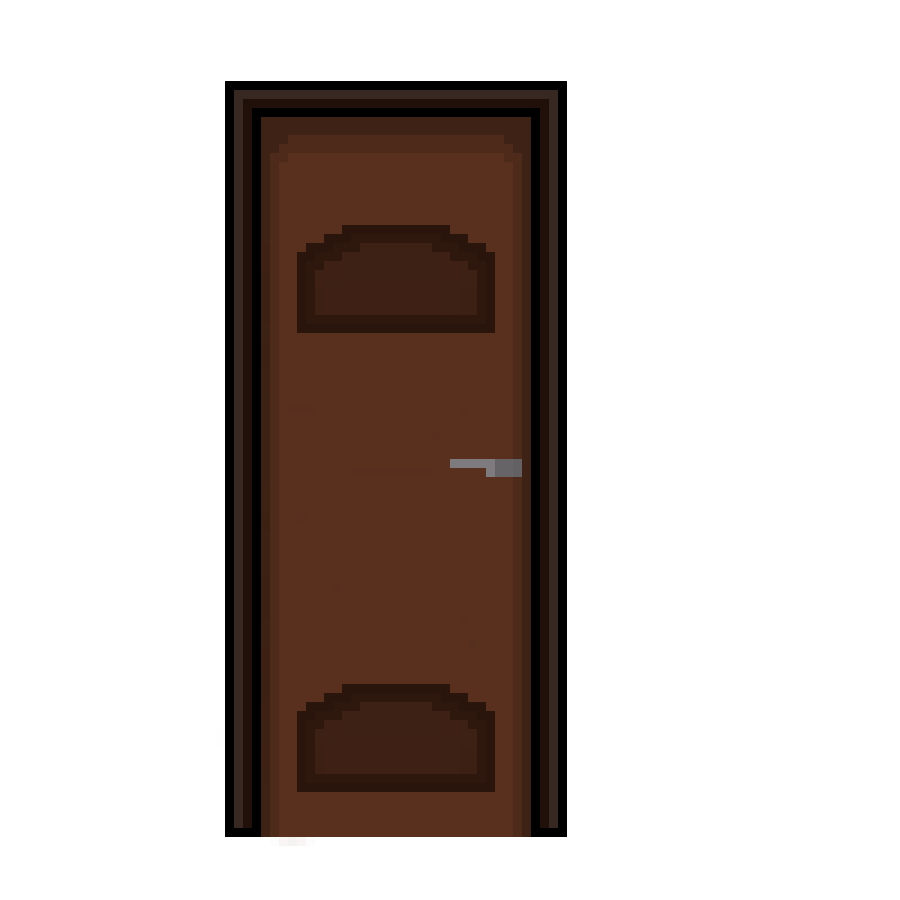
\includegraphics[width=1\linewidth]{figs/vidu/referencia_porta (1).png}
        \caption{\small Sprite da porta em front view}
        \label{fig:geminiProPortaA}
    \end{subfigure}
    \begin{subfigure}{0.23\linewidth}
        \centering
        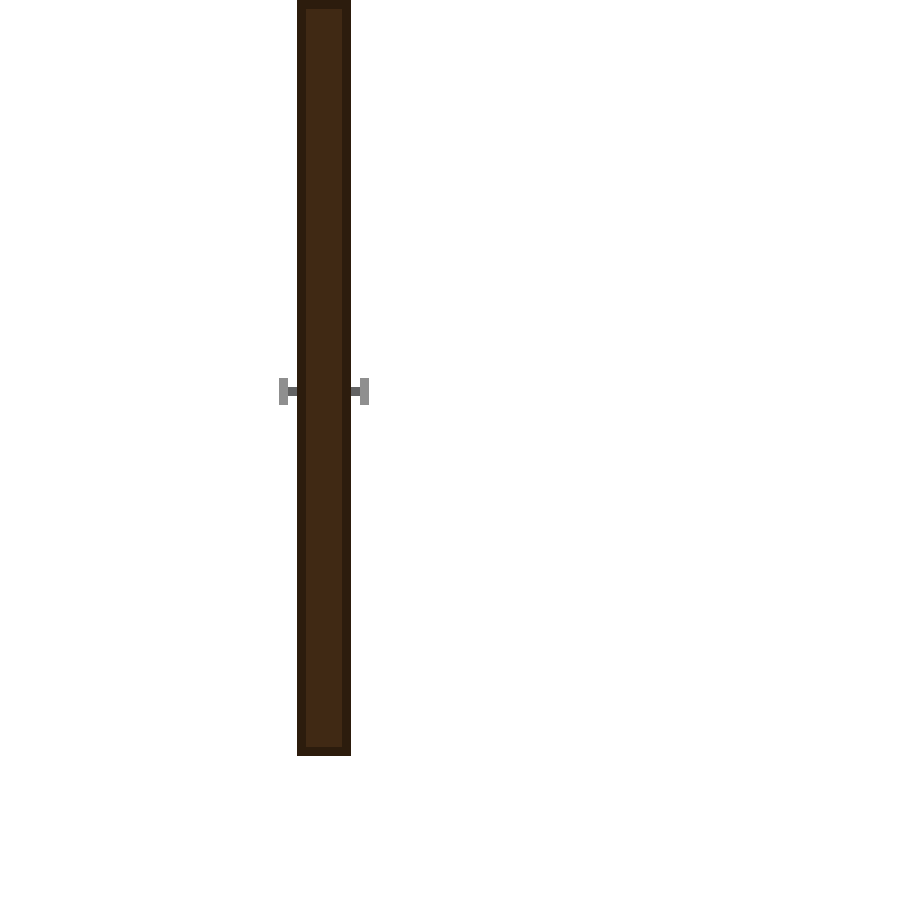
\includegraphics[width=1\linewidth]{figs/vidu/referencia_porta (2).png}
        \caption{\small Sprite da porta em side view}
        \label{fig:geminiProPortaB}
    \end{subfigure}
    % \begin{subfigure}{0.23\linewidth}
    %     \centering
    %     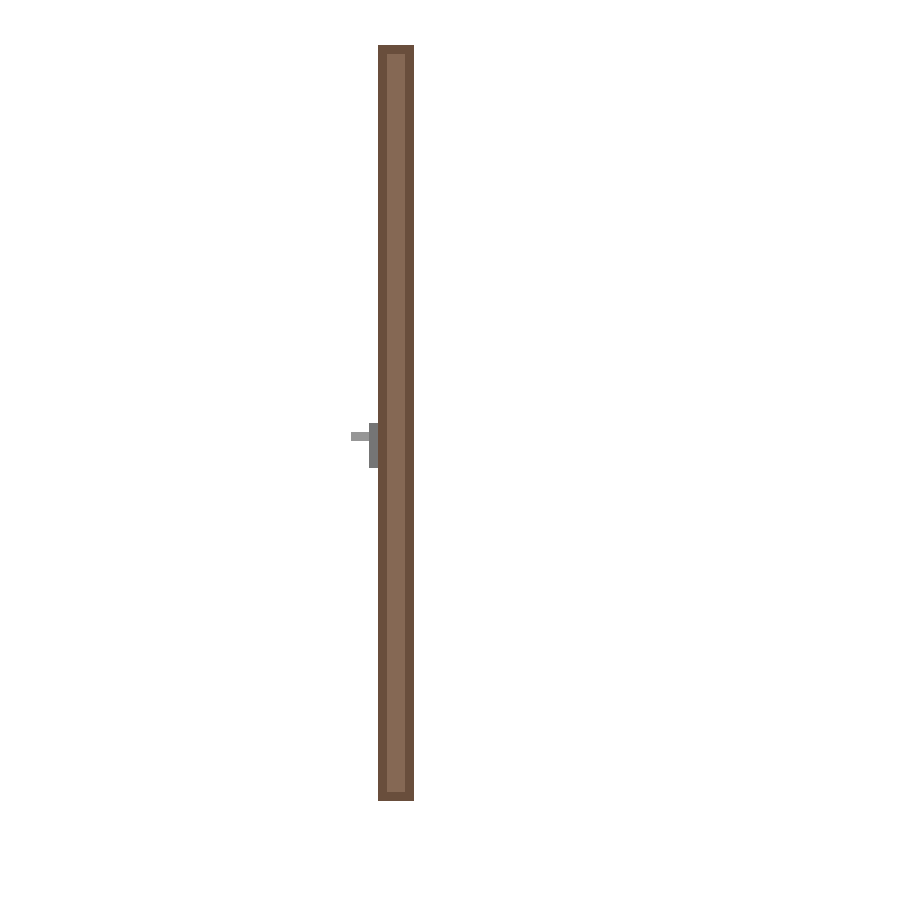
\includegraphics[width=1\linewidth]{figs/vidu/referencia_porta_tutorial (2).png}
    %     \caption{\small Sprite da porta C fechada}
    %     \label{fig:geminiProPortaC2}
    % \end{subfigure}
    % \begin{subfigure}{0.23\linewidth}
    %     \centering
    %     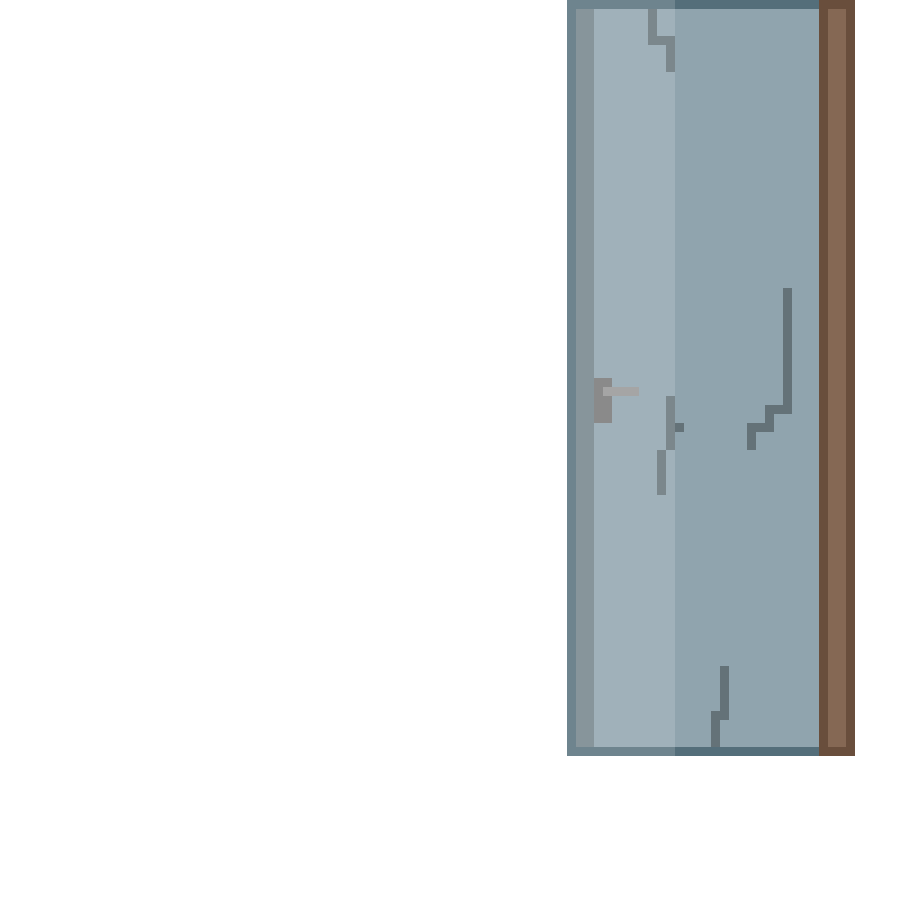
\includegraphics[width=1\linewidth]{figs/vidu/referencia_porta_tutorial (3).png}
    %     \caption{\small Sprite da porta C aberta}
    %     \label{fig:geminiProPortaC3}
    % \end{subfigure}
    % \begin{subfigure}{0.23\linewidth}
    %     \centering
    %     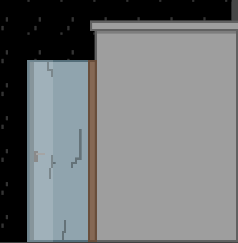
\includegraphics[width=1\linewidth]{figs/sprites/porta.PNG}
    %     \caption{\small Estrutura com porta aberta}
    %     \label{fig:geminiProTutorial}
    % \end{subfigure}
    % \begin{subfigure}{0.23\linewidth}
    %     \centering
    %     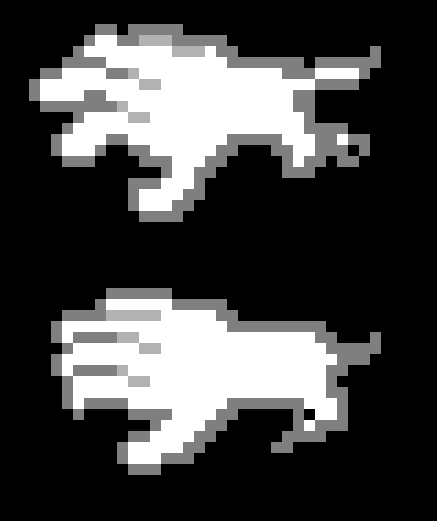
\includegraphics[width=1\linewidth]{figs/sprites/hand.PNG}
    %     \caption{\small Inimigos do jogo}
    %     \label{fig:geminiProMao}
    % \end{subfigure}
    \legend{\small Fonte: Elaborada pela autora.}
\end{figure}

%   ------------------------------------------------------------------------
\FloatBarrier
\subsection{Geração do sprite em side view}
\label{s.gemini.sideview}

Durante os primeiros testes, foi adicionada apenas a imagem do personagem em front view (Figura \ref{fig:geminiProPablo}) junto com o prompt instruindo para rotacionar o personagem em 90 graus. Os resultados mantiveram consistência com o personagem anexado e o estilo, com a maioria deles sendo precisos com a instrução, porém com a parte do rosto apresentando deformações, principalmente em relação aos olhos (que estavam faltando ou muito estreitos). Apenas uma das imagens geradas foi imprecisa, rotacionando o sprite de duas maneiras diferentes (sentido horário e anti-horário) e mostrando ambas (Figura \ref{fig:GeminiProSpriteDuplaRotacao}). Além disso, as imagens visivelmente não estavam no padrão pixel perfect, como é possível de ser visto pelo olho do personagem à esquerda na Figura \ref{fig:GeminiProSpriteDuplaRotacao}. A Figura \ref{fig:GeminiProSpriteSideMelhor1} apresenta o melhor resultado gerado. Interação completa pode ser consultada na Figura \ref{fig:geminiPro1} no Apêndice \ref{ap.telasIA}.

\begin{figure}[htbp]
    \centering
    \begin{minipage}{0.45\textwidth}
        \centering
        \caption{\small Dois sprites em side view gerados em vez de apenas um no Gemini Pro}
        \label{fig:GeminiProSpriteDuplaRotacao}
        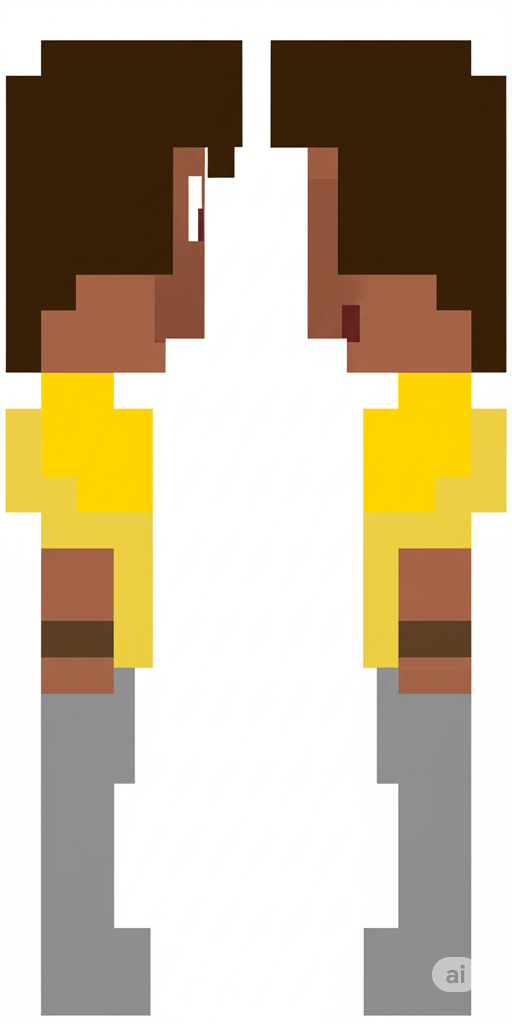
\includegraphics[width=0.5\linewidth]{figs/geminiPro/chat1/res1_tela1.png}
        \legend{\small Fonte: Elaborada pela autora, utilizando a ferramenta Gemini Pro.}
    \end{minipage}\hfill
    \begin{minipage}{0.45\textwidth}
        \centering
        \caption{\small Melhor sprite em side view gerado nos testes iniciais no Gemini Pro}
        \label{fig:GeminiProSpriteSideMelhor1}
        
\includegraphics[width=0.5\linewidth]{figs/geminiPro/chat1/res4_tela1.png}
        \legend{\small Fonte: Elaborada pela autora, utilizando a ferramenta Gemini Pro.}
    \end{minipage}
\end{figure}

Como as deformações mais chamativas estavam na região da cabeça, nos testes posteriores (Figura \ref{fig:geminiPro2}) foram anexadas as Figuras \ref{fig:geminiProPabloChatGPTSide} e \ref{fig:geminiProPabloPixelLab} (até aquele momento, os melhores sprites em side view gerados, respectivamente, pelo ChatGPT e pelo Pixel Lab) para auxiliar especificamente na geração da cabeça. O resultado (Figura \ref{fig:GeminiProSpriteCorpoErrado}) apresentou a cabeça menos deformada, porém apresentou o mesmo erro de formato no corpo que uma das imagens anexadas possuía, além de copiar o fundo com quadrados cinzas dela.

\begin{figure}[htbp]
    \centering
    \caption{\small Sprite gerado em side view com o formato de corpo errado no Gemini Pro}
    \label{fig:GeminiProSpriteCorpoErrado}
    
\includegraphics[width=0.2\linewidth]{figs/geminiPro/chat1/res1_tela2.png}
    \legend{\small Fonte: Elaborada pela autora, utilizando a ferramenta Gemini Pro.}
\end{figure}

No prompt seguinte, a IA foi instruída a manter a cabeça da Figura \ref{fig:GeminiProSpriteCorpoErrado} e o corpo da Figura \ref{fig:GeminiProSpriteSideMelhor1}, porém a ferramenta não gerou um resultado preciso e ainda manteve o fundo quadriculado, como pode ser visto na Figura \ref{fig:GeminiProSpriteFundoCopia}. O teste completo pode ser consultado na Figura \ref{fig:geminiPro3} no Apêndice \ref{ap.telasIA}.

\begin{figure}[htbp]
    \centering
    \caption{\small Sprite gerado em side view com o fundo quadriculado}
    \label{fig:GeminiProSpriteFundoCopia}
    
\includegraphics[width=0.2\linewidth]{figs/geminiPro/chat1/res1_tela3.png}
    \legend{\small Fonte: Elaborada pela autora, utilizando a ferramenta Gemini Pro.}
\end{figure}

Como a imagem do Pixel Lab estava claramente afetando mais do que o esperado os resultados, foi criado um novo chat para novamente gerar imagens sem essa influência no contexto da IA. Foi anexado o sprite em front view e escrito o prompt para rotacionar o personagem. Os resultados gerados foram satisfatórios, apresentando uma performance bem melhor em relação ao primeiro teste, apesar dos prompts serem quase idênticos, como pode ser visto nas Figuras \ref{fig:geminiProSideComparaPrompt} e \ref{fig:geminiProSideComparaMelhor}. Vale destacar que visivelmente nenhum resultado apresentou o padrão pixel perfect. A interação pode ser vista na Figura \ref{fig:geminiPro4} no Apêndice \ref{ap.telasIA}.

\begin{figure}[htbp]
    \centering
    \caption{\small Comparação dos prompts utilizados para geração do sprite em side view usando apenas o front view de referência no Gemini Pro}
    \label{fig:geminiProSideComparaPrompt}
    \begin{subfigure}{0.45\linewidth}
        
\includegraphics[width=1\linewidth]{figs/geminiPro/chat1/prompt.PNG}
        \caption{\small Prompt utilizado nas gerações com o rosto deformado}
        \label{fig:geminiProSideCompararPrompt1}
    \end{subfigure}\hfill
    \begin{subfigure}{0.45 \linewidth}
        \centering
        
\includegraphics[width=1\linewidth]{figs/geminiPro/chat2/prompt.PNG}
        \caption{\small Prompt utilizado nas gerações satisfatórias}
        \label{fig:geminiProSideCompararPrompt2}
    \end{subfigure}
    \legend{\small Fonte: Elaborada pela autora.}
\end{figure}

\begin{figure}[htbp]
    \centering
    \caption{\small Comparação dos resultados em side view usando apenas o front view de referência no Gemini Pro}
    \label{fig:geminiProSideComparaMelhor}
    \begin{subfigure}{0.45\linewidth}
        
\includegraphics[width=0.7\linewidth]{figs/geminiPro/chat1/res4_tela1.png}
        \caption{\small Melhor resultado do teste inicial no primeiro chat}
        \label{fig:geminiProSideCompararMelhor1}
    \end{subfigure}\hfill
    \begin{subfigure}{0.45 \linewidth}
        \centering
        
\includegraphics[width=0.7\linewidth]{figs/geminiPro/chat2/res1_tela1.png}
        \caption{\small Melhor resultado do teste inicial no segundo chat}
        \label{fig:geminiProSideCompararMelhor2}
    \end{subfigure}
    \legend{\small Fonte: Elaborada pela autora.}
\end{figure}

Numa tentativa de verificar se a ferramenta era capaz de produzir um resultado ainda melhor, foi usada a Figura \ref{fig:geminiProSideCompararMelhor2} como referência de como as próximas rotações deveriam ficar. Os sprites gerados apresentaram uma performance pior, com erros na rotação e deformações no rosto. Essa interação é demonstrada na Figura \ref{fig:geminiPro5} no Apêndice \ref{ap.telasIA}.

Mais alguns testes foram feitos para entender quais mudanças no prompt e nos arquivos enviados poderiam aumentar ou diminuir a qualidade dos sprites gerados. 

Adicionar a descrição do personagem não trouxe nenhuma mudança significativa na qualidade dos resultados, gerando inclusive outros resultados satisfatórios, como pode ser visto na Figura \ref{fig:geminiProSideMelhorDescricao}. Os testes com a descrição adicionada ao prompt podem ser consultados nas Figuras \ref{fig:geminiPro6} a \ref{fig:geminiPro9}.

\begin{figure}[htbp]
    \centering
    \caption{\small Melhores resultados em side view adicionando a descrição do personagem no Gemini Pro}
    \label{fig:geminiProSideMelhorDescricao}
    \begin{subfigure}{0.45\linewidth}
        
\includegraphics[width=0.7\linewidth]{figs/geminiPro/chat2/res1_tela3.png}
        \caption{\small Resultado 1}
        \label{fig:geminiProSideMelhorDescricao1}
    \end{subfigure}\hfill
    \begin{subfigure}{0.45 \linewidth}
        \centering
        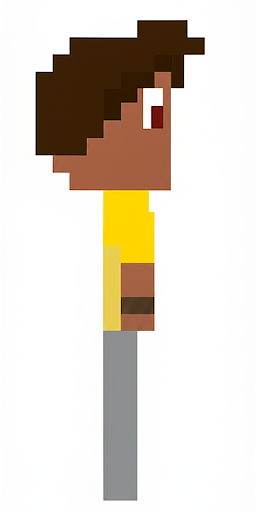
\includegraphics[width=0.7\linewidth]{figs/geminiPro/chat5/tela3_res2.PNG}
        \caption{\small Resultado 2}
        \label{fig:geminiProSideMelhorDescricao2}
    \end{subfigure}
    \legend{\small Fonte: Elaborada pela autora.}
\end{figure}

Escrever um prompt instruindo a ferramenta a fazer o sprite do personagem olhando para a direita e adicionar mais imagens de referências (Figuras \ref{fig:geminiProPablo} a \ref{fig:geminiProPabloPixelLab45_2}), dando o contexto do que cada figura representa em diferentes mensagens, fez com que a IA gerasse um sprite inconsistente com o estilo de pixel art (Figura \ref{fig:GeminiProInconsistenteMelhor}). Ao observar o raciocínio da IA (Figura \ref{fig:GeminiProRaciocinioGeracaoImagem}), foi descoberto que o Gemini apenas formula um prompt para ser enviado ao modelo especializado na geração de imagens, que na época era o Imagen 4. Com isso, foi levantada a hipótese de que, como os sprites de referência foram anexados numa mensagem anterior, o modelo de chat não estava passando essas figuras para o Imagen 4 na hora de gerar a imagem. Para confirmar isso, a ideia era comparar o raciocínio da geração consistente com a da inconsistente, porém em nenhuma das imagens consistentes havia a opção de mostrar os pensamentos. Dessa forma, não foi possível testar a validade da teoria. As Figuras \ref{fig:geminiPro10} a \ref{fig:geminiPro13} no Apêndice \ref{ap.telasIA} demonstram esta bateria de testes.

\begin{figure}[htbp]
    \centering
    \caption{\small Melhor resultado em side view utilizando múltiplas imagens de referência e um contexto maior no Gemini Pro}
    \label{fig:GeminiProInconsistenteMelhor}
    
\includegraphics[width=0.2\linewidth]{figs/geminiPro/chat4/res1_tela16.png}
    \legend{\small Fonte: Elaborada pela autora, utilizando a ferramenta Gemini Pro.}
\end{figure}

\begin{figure}[htbp]
    \centering
    \caption{\small Raciocínio do Gemini Pro antes de gerar a imagem}
    \label{fig:GeminiProRaciocinioGeracaoImagem}
    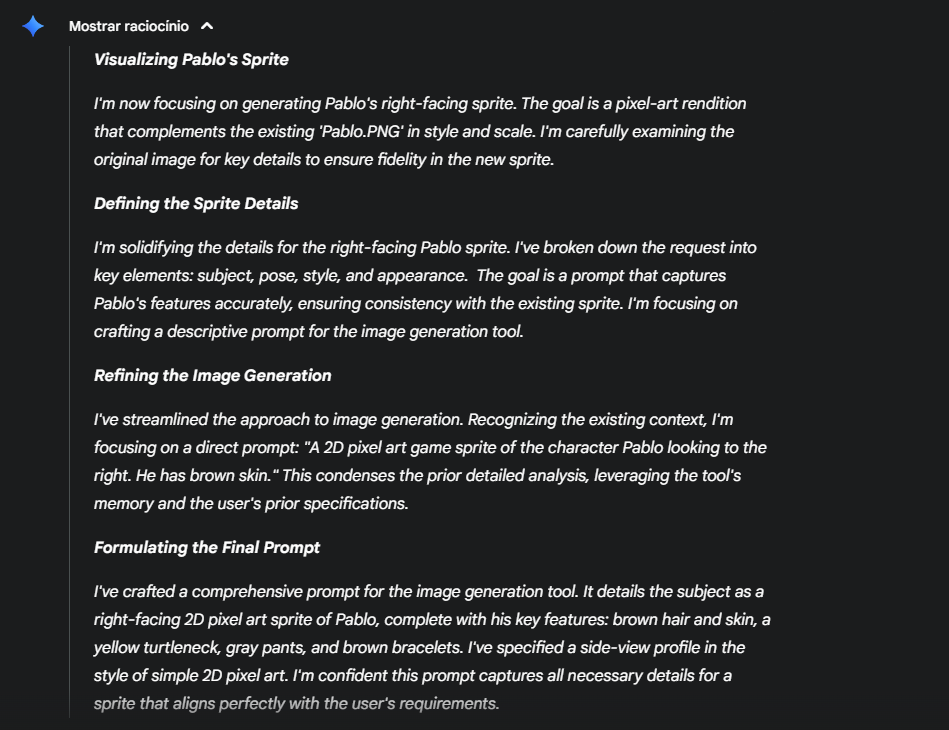
\includegraphics[width=0.8\linewidth]{figs/geminiPro/chat4/tela5.PNG}
    \legend{\small Fonte: Elaborada pela autora.}
\end{figure}

Utilizar como referência o sprite rotacionado em 45 graus (Figura \ref{fig:geminiProPabloPixelLab45_2}), com o prompt pedindo uma rotação de 45 graus para o personagem ficar em side view, gerou o personagem na visão incorreta, como pode ser visto na Figura \ref{fig:GeminiPro45Melhor}. Essa interação pode ser verificada nas Figuras \ref{fig:geminiPro14} a \ref{fig:geminiPro16} no Apêndice \ref{ap.telasIA}.

\begin{figure}[htbp]
    \centering
    \caption{\small Resultado em side view utilizando o sprite rotacionado em 45 graus como referência no Gemini Pro}
    \label{fig:GeminiPro45Melhor}
    
\includegraphics[width=0.2\linewidth]{figs/geminiPro/chat5/tela4_res2.png}
    \legend{\small Fonte: Elaborada pela autora, utilizando a ferramenta Gemini Pro.}
\end{figure}

Foi feita uma última tentativa em gerar um sprite ainda melhor do que o anteriormente gerado, focando em redesenhar o personagem utilizando as imagens dele em side view como referência (Figuras \ref{fig:geminiProPabloPixelLab} e \ref{fig:geminiProSideCompararMelhor2}) em vez de realizar a rotação. A ideia era manter a cabeça parecida com a do melhor sprite em side view gerado pelo Gemini Pro até o momento, e manter o corpo com relevo em ambos os lados, como acontecia no melhor sprite em side view gerado pelo Pixel Lab. O resultado gerado inicialmente foi editado na própria ferramenta através de outros prompts, formando a Figura \ref{fig:GeminiProSideMelhor}. O processo completo pode ser consultado nas Figuras \ref{fig:geminiPro17} a \ref{fig:geminiPro19} no Apêndice \ref{ap.telasIA}.

\begin{figure}[htbp]
    \centering
    \caption{\small Melhor resultado em side view gerado pelo Gemini Pro}
    \label{fig:GeminiProSideMelhor}
    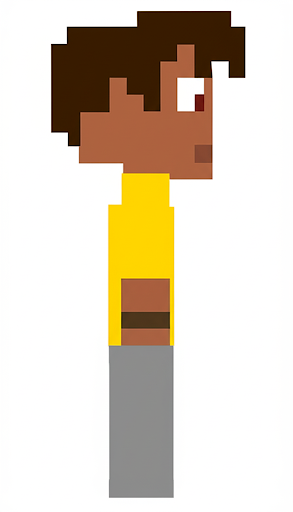
\includegraphics[width=0.3\linewidth]{figs/geminiPro/chat6/tela3_res1.png}
    \legend{\small Fonte: Elaborada pela autora, utilizando a ferramenta Gemini Pro.}
\end{figure}

Posteriormente, essa imagem foi passada para o padrão pixel perfect utilizando o Pixilart (mencionado anteriormente). Ainda dentro do Pixilart, foram feitos pequenos ajustes para corrigir os erros gerados durante a conversão. Esse processo pode ser verificado na Figura \ref{fig:geminiProSideEdicaoMelhor}. Por último, o sprite foi exportado para a ferramenta Pixel Lab, onde mais ajustes foram realizados (detalhados na Seção \ref{s.pixelLab}).

\begin{figure}[htbp]
    \centering
    \caption{\small Processo de edição do melhor sprite em side view no Pixilart}
    \label{fig:geminiProSideEdicaoMelhor}
    \begin{subfigure}{0.32\linewidth}
        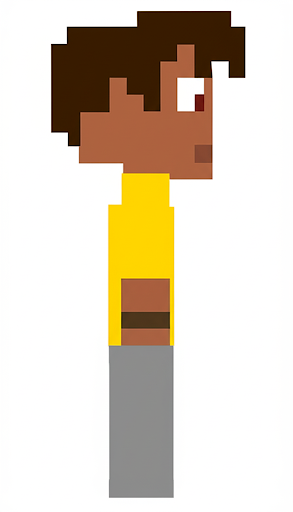
\includegraphics[width=1\linewidth]{figs/geminiPro/chat6/tela3_res1.png}
        \caption{\small Melhor sprite em side view gerado pelo Gemini Pro antes de converter para pixel perfect}
        \label{fig:geminiProSideEdicaoMelhorAntesEdicao}
    \end{subfigure}\hfill
    \begin{subfigure}{0.32\linewidth}
        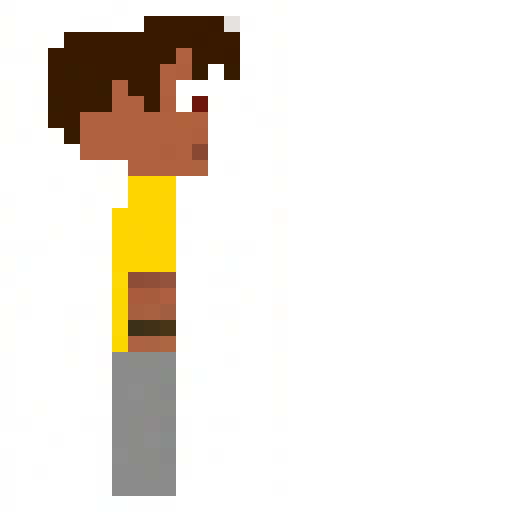
\includegraphics[width=1\linewidth]{figs/geminiPro/passa_pixel_grande.png}
        \caption{\small Sprite em side view após conversão para pixels no Pixilart}
        \label{fig:geminiProSideEdicaoMelhorAposConversao}
    \end{subfigure}\hfill
    \begin{subfigure}{0.32 \linewidth}
        \centering
        
\includegraphics[width=1\linewidth]{figs/geminiPro/fix grande.png}
        \caption{\small Sprite em side view após edição no Pixilart}
        \label{fig:geminiProSideEdicaoMelhorAposEdicao}
    \end{subfigure}
    \legend{\small Fonte: Elaborada pela autora.}
\end{figure}

Conclui-se que o Gemini Pro demonstrou um desempenho superior em relação às ferramentas anteriores na geração do sprite em side view, mantendo alta consistência com o personagem e o estilo em quase todos os testes e sendo preciso na interpretação dos prompts na maioria dos casos. Apesar disso, os resultados não possuem o padrão pixel perfect e a eficácia da IA é sensível ao contexto da conversa, o que pode exigir a criação de novos chats para evitar uma repetição de erros. Embora a edição de imagens diretamente na plataforma seja limitada ao uso da IA, a capacidade dessa ferramenta em gerar um desenho base coeso e de alta qualidade solidifica seu papel na eficiência na produção de poses para auxílio no processo de animação.


%   ------------------------------------------------------------------------
\FloatBarrier
\subsection{Geração do sprite em back view}
\label{s.gemini.backview}

Para a geração do sprite em back view, foi usado como referência o sprite em front view (Figura \ref{fig:geminiProPablo}) e o sprite em side view (Figura \ref{fig:geminiProSideEdicaoMelhorAposEdicao}). Inicialmente, o modelo interpretou errado a instrução de fazer o personagem virado para o norte, gerando o sprite em front view com deformações de pixels no rosto, que aparentavam formar um sorriso. Isso pode ser visto na Figura \ref{fig:GeminiProSpriteSegundoRosto}.

\begin{figure}[htbp]
    \centering
    \caption{\small Sprite gerado em back view com pixels errados no rosto no Gemini Pro}
    \label{fig:GeminiProSpriteSegundoRosto}
    
\includegraphics[width=0.3\linewidth]{figs/geminiPro/chat12/01_res2.png}
    \legend{\small Fonte: Elaborada pela autora, utilizando a ferramenta Gemini Pro.}
\end{figure}

Na interação seguinte, foi especificado melhor que o personagem deveria estar de costas. Os resultados gerados foram todos satisfatórios, mantendo alta consistência com o estilo e o personagem, como pode ser visto na Figura \ref{fig:GeminiProBackMelhor}. A olho nu, os sprites parecem manter o padrão pixel perfect, sendo facilmente exportados para aplicativos de edição de pixel art.

\begin{figure}[htbp]
    \centering
    \caption{\small Melhor sprite gerado em back view no Gemini Pro}
    \label{fig:GeminiProBackMelhor}
    
\includegraphics[width=0.3\linewidth]{figs/geminiPro/chat12/02_res2.png}
    \legend{\small Fonte: Elaborada pela autora, utilizando a ferramenta Gemini Pro.}
\end{figure}

Apesar disso, foi notado que os tons de cores não eram exatamente idênticos aos do sprite original, sendo necessário que a imagem passasse por essa correção. Assim como foi feito com o sprite em side view, a imagem foi exportada para o Pixilart, como pode ser visto na Figura \ref{fig:geminiProBackEdicaoMelhor}. Após isso, a imagem foi colocada na ferramenta Pixel Lab, onde foi realizado o pós-processamento (detalhado na Seção \ref{s.pixelLab}).

\begin{figure}[htbp]
    \centering
    \caption{\small Processo de edição do melhor sprite em back view no Pixirart}
    \label{fig:geminiProBackEdicaoMelhor}
    \begin{subfigure}{0.45\linewidth}
        
\includegraphics[width=1\linewidth]{figs/geminiPro/chat12/02_res2.png}
        \caption{\small Melhor sprite em back view gerado pelo Gemini Pro antes de converter para pixel perfect}
        \label{fig:geminiProBackEdicaoMelhorAntesEdicao}
    \end{subfigure}\hfill
    \begin{subfigure}{0.45\linewidth}
        
\includegraphics[width=1\linewidth]{figs/geminiPro/back_pixel_grande.png}
        \caption{\small Sprite em back view após conversão para pixels no Pixilart}
        \label{fig:geminiProBackEdicaoMelhorAposConversao}
    \end{subfigure}\hfill
    \legend{\small Fonte: Elaborada pela autora.}
\end{figure}

Os resultados dos testes descritos nesta seção podem ser consultados nas Figuras \ref{fig:geminiProBack1} e \ref{fig:geminiProBack2}.

Em geral, os testes para a geração do sprite em back view revelaram uma capacidade de consistência ainda maior do que a observada anteriormente. O modelo foi capaz de simular o padrão pixel perfect com alta fidelidade a olho nu, um feito impressionante para um modelo de IA generativo que não é especializado nesse estilo, solidificando ainda mais o Gemini Pro como a ferramenta mais eficiente para a criação de poses base para animações 2D.


%   ------------------------------------------------------------------------
\FloatBarrier
\subsection{Geração do sprite sheet do ciclo de caminhada}
\label{s.gemini.spritesheet}

No teste inicial (Figura \ref{fig:geminiProSheet1} no Apêndice \ref{ap.telasIA}), foi anexado o personagem em front view (Figura \ref{fig:geminiProPablo}) e o melhor sprite gerado até aquele momento em side view (Figura \ref{fig:GeminiProSpriteSheetSide}) junto com a descrição do personagem e o contexto de cada imagem. Apenas na mensagem posterior foi enviado o prompt instruindo a ferramenta a gerar o sprite sheet com 16 frames. Isso foi feito para verificar se o erro de consistência (descrito na Seção \ref{s.gemini.sideview}) ocorreria novamente. 

\begin{figure}[htbp]
    \centering
    \caption{\small Sprite em side view usado como referência no teste inicial da geração do sprite sheet no Gemini Pro}
    \label{fig:GeminiProSpriteSheetSide}
    
\includegraphics[width=0.3\linewidth]{figs/geminiPro/chat6/tela2_res4.png}
    \legend{\small Fonte: Elaborada pela autora, utilizando a ferramenta Gemini Pro.}
\end{figure}

Como esperado, os resultados demonstraram inconsistência com o estilo, como se estivessem usando como base apenas as características do personagem e ignorando as imagens de referência, o que pode ser visto na Figura \ref{fig:GeminiProSpriteSheetInconsistente}. Isso contribui para a hipótese anterior, sobre o modelo de chat estar enviando apenas o prompt textual para o Imagen 4 por causa do envio das imagens numa mensagem diferente. Para consolidar essa teoria, mais testes foram realizados utilizando um prompt idêntico com a imagem anexada na mesma mensagem. Porém, antes de abordar esses novos experimentos, é importante ressaltar outras características presentes em todas as figuras geradas. A IA foi capaz de fazer 16 quadros, porém — como aconteceu durante a análise de outras ferramentas — o mesmo sprite era repetido com mudanças não significativas, sem formar o movimento de caminhada. 


\begin{figure}[htbp]
    \centering
    \caption{\small Sprite sheet inconsistente gerado no Gemini Pro}
    \label{fig:GeminiProSpriteSheetInconsistente}
    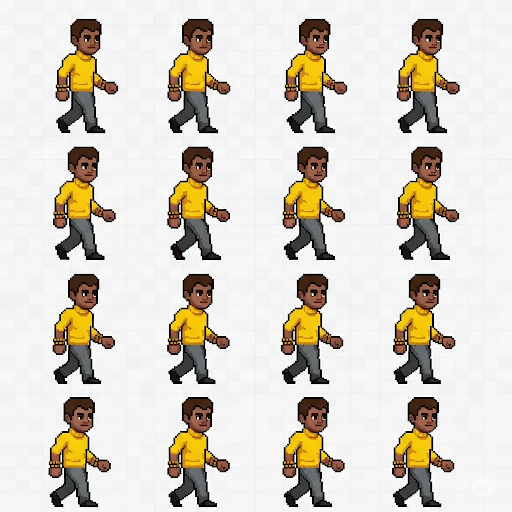
\includegraphics[width=0.5\linewidth]{figs/geminiPro/chat8/tela1_res5.PNG}
    \legend{\small Fonte: Elaborada pela autora, utilizando a ferramenta Gemini Pro.}
\end{figure}

Continuando os testes, foi anexada a melhor imagem do personagem em side view gerada (que naquele momento era a Figura \ref{fig:GeminiProSideMelhor}) e repetido o mesmo prompt de antes. De maneira inesperada, os resultados apresentaram consistência variável com o estilo, como pode ser visto na Figura \ref{fig:GeminiProSpriteSheetConsistenciaVariavel}. Além disso, o número de quadros gerados foi diferente do valor instruído, possuindo diversos frames repetidos, porém eventualmente mudando a pose para avançar o movimento (o que não ocorreu na geração anterior). Todos os resultados podem ser consultados na Figura \ref{fig:geminiProSheet2} no Apêndice \ref{ap.telasIA}.

\begin{figure}[htbp]
    \centering
    \caption{\small Sprite sheet parcialmente inconsistente gerado no Gemini Pro}
    \label{fig:GeminiProSpriteSheetConsistenciaVariavel}
    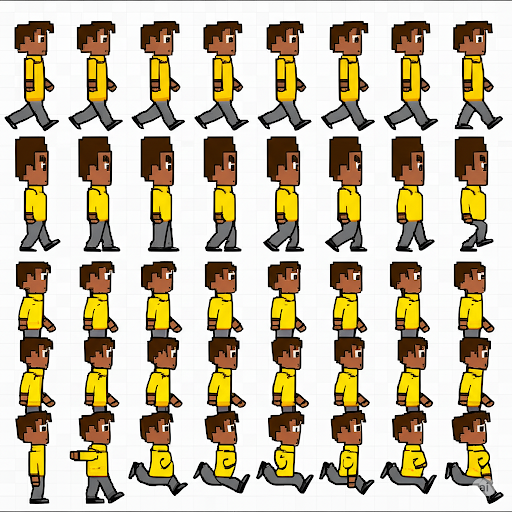
\includegraphics[width=0.5\linewidth]{figs/geminiPro/chat8/tela2_res1.PNG}
    \legend{\small Fonte: Elaborada pela autora, utilizando a ferramenta Gemini Pro.}
\end{figure}

Analisando a fundo, foi levantada a teoria de que os resultados podem ter sido influenciados pelo contexto já existente da ferramenta, pois ambas as baterias de testes foram realizadas no mesmo chat. Isso explicaria o motivo de algumas imagens geradas manterem a consistência com a figura anexada, enquanto outras apresentavam a mesma inconsistência do experimento anterior. Para eliminar essa interferência, foi criado um novo chat, onde replicou-se de maneira exata o teste inicial (utilizando as Figuras \ref{fig:geminiProPablo} e \ref{fig:GeminiProSpriteSheetSide}), exceto pelo fato de que os textos (descrição, contexto e prompt) foram unidos em uma só mensagem. 

Os resultados apresentaram uma consistência maior do que os testes anteriores, mantendo características específicas das referências, porém perdendo o estilo de pixel art e com diversas deformações no sprite, como pode ser visto na Figura \ref{fig:GeminiProSpriteSheetMelhor1}. O erro de frames sem mudanças significativas diminuiu, porém foram gerados mais do que 16 quadros e algumas posições apareceram de forma imprecisa . Em alguns casos, o personagem era desconstruído ou parecia fazer ações diferentes do que apenas andar, como pode ser observado na Figura \ref{fig:GeminiProSpriteSheetDesconstruido}. Em geral, apesar de mostrarem uma semelhança maior com o estilo da imagem de referência, os resultados foram menos precisos, com mais deformações e menos satisfatórios quando considerada apenas a descrição textual do personagem. A interação completa pode ser consultada na Figura \ref{fig:geminiPro3} no Apêndice \ref{ap.telasIA}.

\begin{figure}[htbp]
    \centering
    \caption{\small Melhor sprite sheet do personagem andando utilizando várias imagens de referência na mesma mensagem do prompt gerado no Gemini Pro}
    \label{fig:GeminiProSpriteSheetMelhor1}
    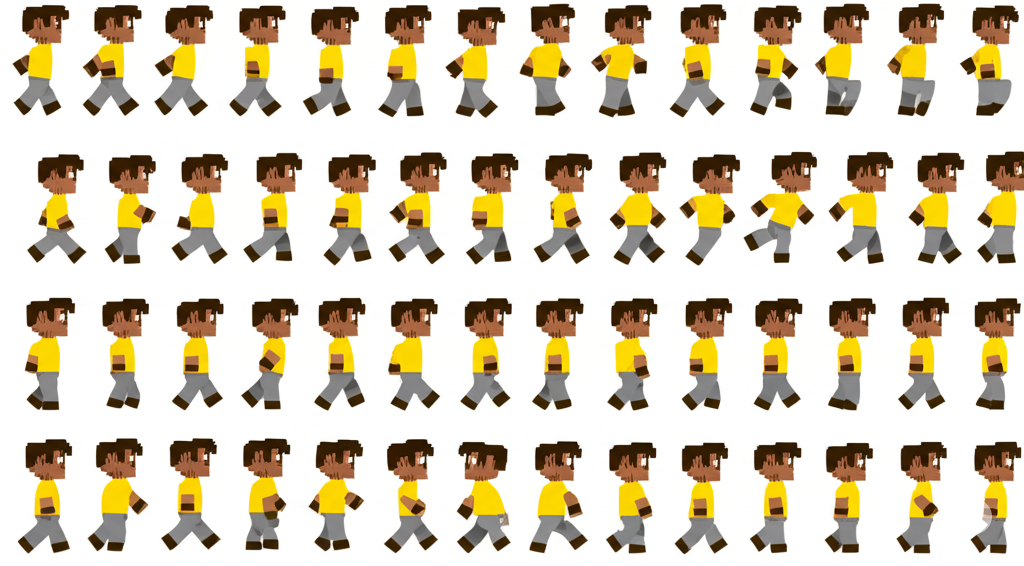
\includegraphics[width=0.8\linewidth]{figs/geminiPro/chat9/1res1.PNG}
    \legend{\small Fonte: Elaborada pela autora, utilizando a ferramenta Gemini Pro.}
\end{figure}

\begin{figure}[htbp]
    \centering
    \caption{\small Sprite sheet com o personagem mantendo diferentes partes do desenho gerado no Gemini Pro}
    \label{fig:GeminiProSpriteSheetDesconstruido}
    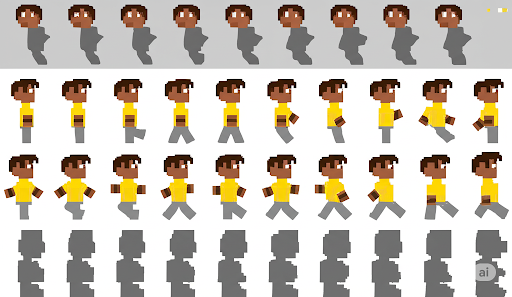
\includegraphics[width=0.6\linewidth]{figs/geminiPro/chat9/1res5.PNG}
    \legend{\small Fonte: Elaborada pela autora, utilizando a ferramenta Gemini Pro.}
\end{figure}

Nos testes seguintes, voltou-se a anexar apenas a melhor imagem gerada em side view até aquele momento (Figura \ref{fig:GeminiProSideMelhor}). 

Quando era usado o mesmo chat, geraram-se sprites mais parecidos com o de referência e com levemente menos deformações, porém ainda mantendo as demais características comentadas anteriormente (Figura \ref{fig:geminiPro4} no Apêndice \ref{ap.telasIA}). 

Entretanto, ao se utilizar um novo chat, a consistência do personagem e do estilo aumentou de forma satisfatória na maioria das figuras geradas, com um número menor de deformações em comparação com os outros resultados, como pode ser visto na Figura \ref{fig:GeminiProSpriteSheetMelhor}. De maneira inesperada, essa estratégia gerou, em certos momentos, sequências de imagens com os sprites em vez de uma imagem com o sprite sheet, além de apresentar uma maior repetição de quadros sem mudança significativa.  Os resultados completos podem ser verificados na Figura \ref{fig:geminiPro5} no Apêndice \ref{ap.telasIA}.

\begin{figure}[htbp]
    \centering
    \caption{\small Melhor sprite sheet gerado no Gemini Pro}
    \label{fig:GeminiProSpriteSheetMelhor}
    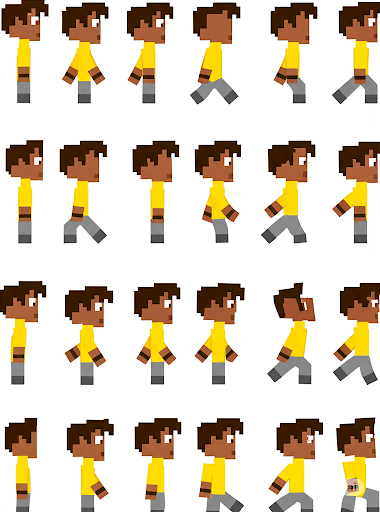
\includegraphics[width=0.5\linewidth]{figs/geminiPro/chat10/tela1_res3.PNG}
    \legend{\small Fonte: Elaborada pela autora, utilizando a ferramenta Gemini Pro.}
\end{figure}

\begin{quadro}[htbp]
    \centering
    \caption{\small Resumo dos experimentos de geração do sprite sheet no Gemini Pro}
    \label{quadro:GeminiProSpriteSheet}
    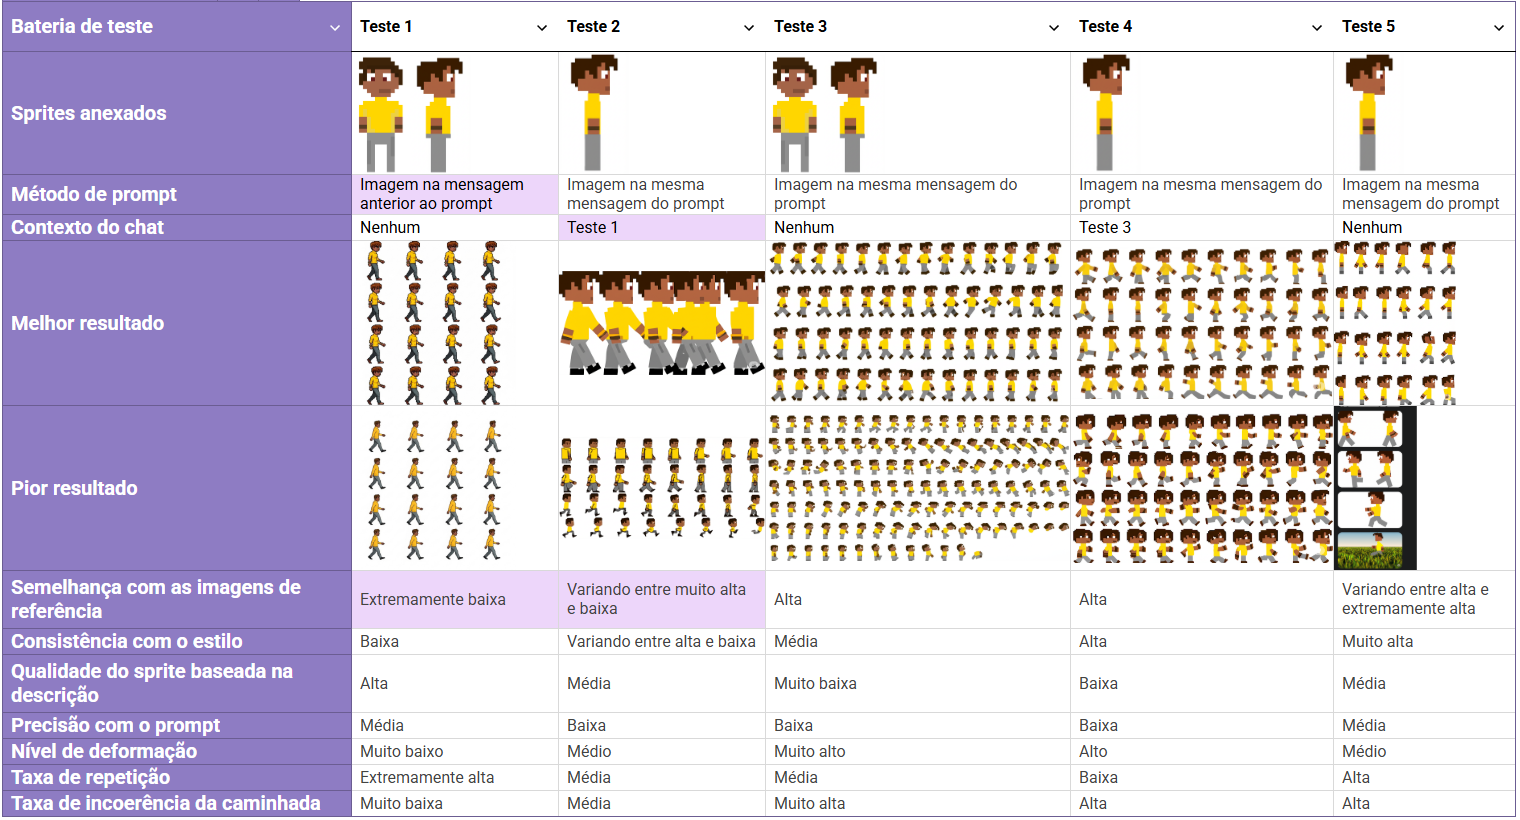
\includegraphics[width=1\linewidth]{figs/geminiPro/tabela_geracao_sprite_sheet.PNG}
    \legend{\small Fonte: Elaborada pela autora.}
\end{quadro}


Analisando e comparando todos os resultados, compilados no Quadro \ref{quadro:GeminiProSpriteSheet}, é consolidada a hipótese sobre a importância de anexar as imagens de referência na mesma mensagem do prompt. A provável causa desse comportamento é que o modelo de chat não retém o conteúdo visual de mensagens anteriores que não tiverem relação com uma geração da imagem, dessa forma não podendo enviar a figura ao formular a instrução para o Imagen 4.

Os experimentos também revelaram que a ferramenta Gemini Pro apresenta dificuldades em gerar sequências de imagens com pequenas variações. A IA tende a repetir quadros e poses, introduzir deformações ou perder a precisão da progressão do movimento ao tentar criar os múltiplos sprites de uma animação. Conclui-se que, embora excelente para a criação de sprites específicos, o Gemini Pro não se mostrou capaz de formar o sprite sheet de uma animação, falhando em compreender o contexto temporal de um ciclo de caminhada.


%   ------------------------------------------------------------------------
\FloatBarrier
\subsection{Geração da animação de caminhada}
\label{s.gemini.animacaoAndar}

Como comentado anteriormente, a geração de vídeo era limitada a três animações por dia. Esse fator fez com que, antes mesmo de ter o sprite final em side view do personagem, fossem realizados testes para produzir o movimento de caminhada. Só era possível anexar uma única imagem e o prompt tinha que ser reescrito novamente a cada resultado gerado. Todos os vídeos produzidos possuem som, porém o foco da análise foi especificamente no conteúdo visual produzido, sem levar em conta o material sonoro.


Durante os testes iniciais (Figuras \ref{fig:geminiProAndar1} e \ref{fig:geminiProAndar2} no Apêndice \ref{ap.telasIA}), foi utilizado o sprite do personagem em front view como imagem a ser transformada em vídeo. Os resultados\footnote{\url{https://drive.google.com/drive/folders/1rbBwuVsgvShD8JoruLJN_poLJRwVSOcO?usp=sharing}} gerados mantiveram em grande parte a pixel art, criaram precisamente o movimento de caminhada e formaram o sprite em side view consistente com o estilo, porém apresentando incongruências em relação a características físicas específicas e aos tons de cores (Figura \ref{fig:GeminiProAndarComparaSprite}). Um detalhe interessante de ser ressaltado foi que, diferente das outras ferramentas de vídeo, a animação não deformou completamente a pixel art, como pode ser visto na Figura \ref{fig:geminiProAndarQuadroPixelCoerente}. Apesar da alta qualidade, a inconsistência chamativa na aparência fez com que esses vídeos não fossem considerados satisfatórios para a animação no jogo.

\begin{figure}[htbp]
    \centering
    \caption{\small Comparação do sprite em front view com os sprites em side view das animações geradas no Gemini Pro}
    \label{fig:GeminiProAndarComparaSprite}
    \begin{subfigure}{0.32\linewidth}
        \centering
        
\includegraphics[width=0.7\linewidth]{figs/sprites/Pablo.PNG}
        \caption{\small Sprite do Pablo em front view, sem sapato visível}
        \label{fig:GeminiProAndaPablo}
    \end{subfigure}
    \begin{subfigure}{0.32\linewidth}
        \centering
        
\includegraphics[width=0.7\linewidth]{figs/geminiPro/chat3/sprite1.PNG}
        \caption{\small Sprite com adição de sapatos pretos e olhos de cor e tamanho diferente da referência}
        \label{fig:GeminiProAndarComparaSprite1}
    \end{subfigure}
    \begin{subfigure}{0.32\linewidth}
        \centering
        
\includegraphics[width=0.7\linewidth]{figs/geminiPro/chat3/sprite2.PNG}
        \caption{\small Sprite com olho maior que a referência e pupila de dois tons de cores}
        \label{fig:GeminiProAndarComparaSprite2}
    \end{subfigure}

    \legend{\small Fonte: Elaborada pela autora, utilizando a ferramenta Gemini Pro.}
\end{figure}

\begin{figure}[htbp]
    \centering
    \caption{\small Quadro da animação de caminhada gerada no Gemini Pro, circulada em vermelho a diagonal incoerente com pixel art e circulada em azul a diagonal pixelizada de forma coerente}
    \label{fig:geminiProAndarQuadroPixelCoerente}
    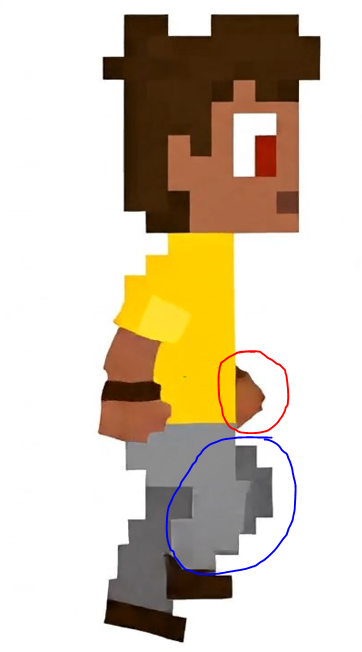
\includegraphics[width=0.3\linewidth]{figs/geminiPro/chat3/animacaoPixelArt.PNG}
    \legend{\small Fonte: Elaborada pela autora, utilizando a ferramenta Gemini Pro.}
\end{figure}

No teste seguinte (Figura \ref{fig:geminiProAndar3} no Apêndice \ref{ap.telasIA}), foi anexado o melhor sprite em side view que havia até aquele momento (Figura \ref{geminiProSideCompararMelhor2}), fazendo com que não se precisasse gerar um sprite em side view junto com o vídeo, sendo necessário produzir apenas a animação. O resultado\footnote{\url{https://drive.google.com/file/d/1dQZF4InImDsFU4jw68rXUGffW1hfGMWA/view?usp=sharing}} foi extremamente consistente com a referência e apresentou o movimento correto de andar. A animação deforma a pixel art de modo a formar diagonais incoerentes, porém essa falha não foi muito chamativa. Apesar disso, o vídeo possuía um erro grave que tornava o mesmo inadequado para uso: durante a animação, quando o braço se move, é revelado um buraco nas costas. Isso pode ser visto na Figura \ref{fig:GeminiProAndarFuroCostas}. 
\begin{figure}[htbp]
    \centering
    \caption{\small Comparação do sprite em side view de referência com o sprite da animação gerada no Gemini Pro}
    \label{fig:GeminiProAndarFuroCostas}
    \begin{subfigure}{0.45\linewidth}
        \centering
        
\includegraphics[width=0.3\linewidth]{figs/geminiPro/chat2/res1_tela1.png}
        \caption{\small Sprite do Pablo em side view}
        \label{fig:GeminiProAndarFuroCostasReferencia}
    \end{subfigure}
    \begin{subfigure}{0.45\linewidth}
        \centering
        
\includegraphics[width=0.3\linewidth]{figs/geminiPro/chat3/sprite3.PNG}
        \caption{\small Quadro da animação de caminhada revelando o vão nas costas}
        \label{fig:GeminiProAndarFuroCostasResultado}
    \end{subfigure}

    \legend{\small Fonte: Elaborada pela autora, utilizando a ferramenta Gemini Pro.}
\end{figure}

Analisando a imagem de referência, foi teorizado que a maneira em que o sprite estava desenhado foi responsável por fazer com que a IA entendesse que a linha do corpo acabava antes (Figura \ref{fig:geminiProAndarLinhaCorpo}), o que ficava desconectado da perna e criava o vão. 

\begin{figure}[htbp]
    \centering
    \caption{\small Linha preta representando possível interpretação do modelo de IA sobre onde o torso terminava}
    \label{fig:geminiProAndarLinhaCorpo}
    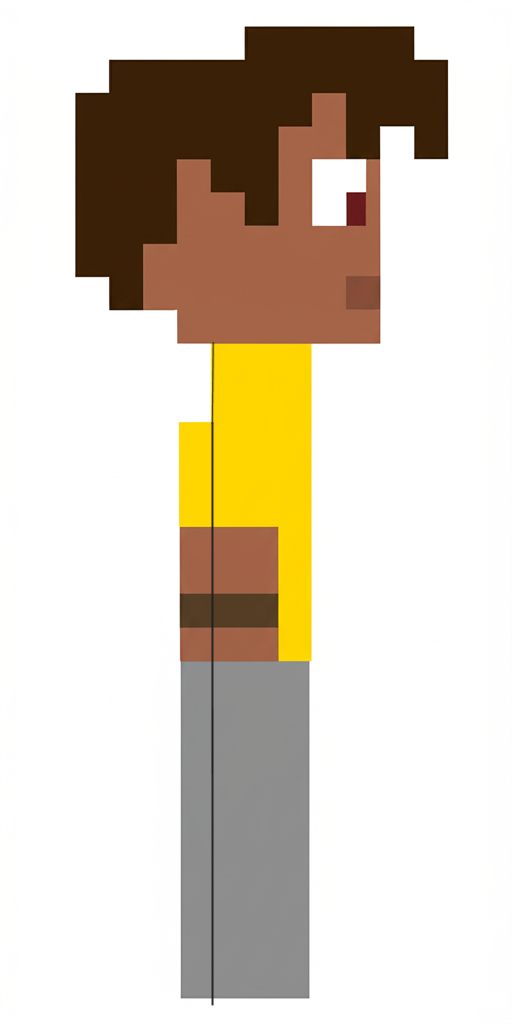
\includegraphics[width=0.3\linewidth]{figs/geminiPro/chat3/linhaCorpo.png}
    \legend{\small Fonte: Elaborada pela autora, utilizando a ferramenta Gemini Pro.}
\end{figure}

Para evitar essa falha, o sprite apresentado abaixo na Figura \ref{fig:GeminiProAndarSide1} foi usado como referência no teste posterior (Figura \ref{fig:geminiProAndar4} no Apêndice \ref{ap.telasIA}). O resultado\footnote{\url{https://drive.google.com/file/d/1Bi-5QSThXMqe6zONrDluai8ukYTAYkVj/view?usp=sharing}} gerado foi satisfatório, apresentando alta consistência e precisão. Apesar disso, o vídeo adicionou sapatos pretos no personagem e apresentou distorções na região dos joelhos e das mãos (Figura \ref{fig:GeminiProAndarDeformacao}, além da animação deformar a pixel art fazendo-a perder a coerência. 

\begin{figure}[htbp]
    \centering
    \begin{minipage}{0.45\textwidth}
        \centering
        \caption{\small Sprite em side view usado como referência na geração da animação no Gemini Pro}
        \label{fig:GeminiProAndarSide1}
        
\includegraphics[width=0.5\linewidth]{figs/geminiPro/chat6/tela2_res4.png}
        \legend{\small Fonte: Elaborada pela autora, utilizando a ferramenta Gemini Pro.}
    \end{minipage}\hfill
    \begin{minipage}{0.45\textwidth}
        \centering
        \caption{\small Quadro da animação gerada no Gemini Pro com distorções circuladas em vermelho}
        \label{fig:GeminiProAndarDeformacao}
        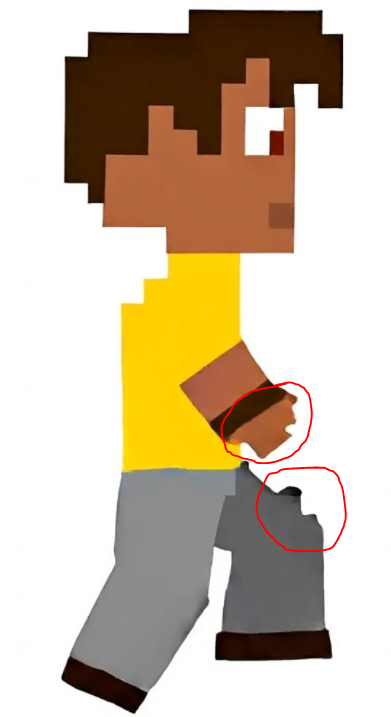
\includegraphics[width=0.5\linewidth]{figs/geminiPro/chat7/deformacoes1.PNG}
        \legend{\small Fonte: Elaborada pela autora, utilizando a ferramenta Gemini Pro.}
    \end{minipage}
\end{figure}

Como foi rapidamente gerada uma animação adequada, os experimentos seguintes focaram em testar se a ferramenta mantém esse alto padrão na geração e se era possível criar um vídeo que não tivesse nenhuma distorção. Para esses testes, uma versão aprimorada do sprite anterior (Figura \ref{fig:GeminiProSideMelhor}) foi utilizada como referência. Os resultados\footnote{\url{https://drive.google.com/drive/folders/19e9IRIDhn1UlBP_wyuXw2AIhyZP0OnSC?usp=sharing}} também foram satisfatórios, apresentando alta consistência e precisão e não possuindo as distorções citadas anteriormente. Porém, ainda foram encontrados pequenos erros de consistência, que podem ser vistos na Figura \ref{fig:GeminiProAndarComparaSpriteSide2}. Apesar disso, um dos vídeos gerados mostrou-se mais adequado do que os prévios, com apenas uma única inconsistência visível (Figura \ref{fig:GeminiProAndarComparaSide2Sprite2}. Os testes completos podem ser consultados nas Figuras \ref{fig:geminiProAndar5} e \ref{fig:geminiProAndar6} no Apêndice \ref{ap.telasIA}. 

\begin{figure}[htbp]
    \centering
    \caption{\small Comparação do sprite de referência com os sprites em side view das animações geradas no Gemini Pro}
    \label{fig:GeminiProAndarComparaSpriteSide2}
    \begin{subfigure}{0.32\linewidth}
        \centering
        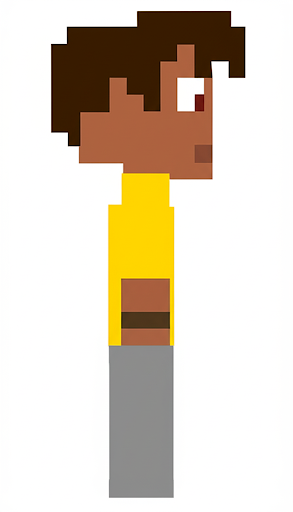
\includegraphics[width=0.7\linewidth]{figs/geminiPro/chat6/tela3_res1.png}
        \caption{\small Sprite do Pablo em side view usado de referência}
        \label{fig:GeminiProAndarSide2}
    \end{subfigure}
    \begin{subfigure}{0.32\linewidth}
        \centering
        \includegraphics[width=0.7\linewidth]{figs/geminiPro/chat7/sprite2.PNG}
        \caption{\small Sprite com inconsistência na boca e no bracelete}
        \label{fig:GeminiProAndarComparaSide2Sprite1}
    \end{subfigure}
    \begin{subfigure}{0.32\linewidth}
        \centering
        \includegraphics[width=0.7\linewidth]{figs/geminiPro/chat7/sprite3.PNG}
        \caption{\small Sprite com inconsistência no sapato}
        \label{fig:GeminiProAndarComparaSide2Sprite2}
    \end{subfigure}

    \legend{\small Fonte: Elaborada pela autora, utilizando a ferramenta Gemini Pro.}
\end{figure}

 Comparando todos os vídeos gerados, foi possível perceber que as animações geradas usando o personagem em front view como referência apresentavam menos incoerências na pixel art em relação aos que usavam um sprite em side view. Foi levantada a hipótese de que a IA consegue gerar de maneira mais precisa a animação em pixel art quando a referência está no padrão pixel perfect. As imagens em side view não estavam nesse padrão pois tinham sido feitas por IA.

Como havia outras animações para serem geradas, foi decidido fazer a implementação do melhor resultado no jogo. Para isso, o vídeo foi transformado em um sprite sheet (Figura \ref{fig:geminiProAndarSpriteSheet}) usando a ferramenta ezgif (mencionada anteriormente).

\begin{figure}[htbp]
    \centering
    \caption{\small Sprite sheet do vídeo de caminhada gerado no Gemini Pro}
    \label{fig:geminiProAndarSpriteSheet}
    \includegraphics[width=0.8\linewidth]{figs/geminiPro/sprite sheet/video3.png}
    \legend{\small Fonte: Elaborada pela autora, utilizando a ferramenta ezgif.}
\end{figure}

Além disso, também foi necessário remover o fundo da imagem para que o mesmo não aparecesse durante o jogo. Para isso, foi utilizada a ferramenta removebg\footnote{\url{https://www.remove.bg/upload}}. O resultado pode ser consultado na Figura \ref{fig:geminiProAndarSpriteSheetSemFundo}.

\begin{figure}[htbp]
    \centering
    \caption{\small Sprite sheet do ciclo de caminhada sem fundo}
    \label{fig:geminiProAndarSpriteSheetSemFundo}
    \includegraphics[width=0.8\linewidth]{figs/geminiPro/sprite sheet/sprite_fundo_transparente3.png}
    \legend{\small Fonte: Elaborada pela autora, utilizando a ferramenta removebg.}
\end{figure}



Posteriormente, o sprite em side view foi ajustado e aprimorado no Pixel Lab, o que tornou ultrapassada a imagem usada na animação de caminhada. As diferenças não eram muito grandes, de maneira que o vídeo ainda fosse adequado para ser usado no jogo. Porém, mesmo assim, novos testes foram realizados com a Figura \ref{fig:geminiProPabloPixelLabSide} de referência. Os resultados\footnote{\url{https://drive.google.com/drive/folders/16IjPYloPZtl81zKZ3kOz3I3qkPX078_9?usp=sharing}} não foram melhores do que a animação já implementada, todos apresentando mais erros de consistência que o anterior, em específico fazendo o bracelete ganhar um relevo que dava uma vaga sensação de 3D, como pode ser visto na Figura \ref{fig:GeminiProAndarBracelete3D}. Diversos prompts diferentes foram usados em busca de corrigir essa falha, porém não houve sucesso. Também é importante notar que alguns dos resultados conseguiram parcialmente manter a coerência da pixel art durante a animação (Figura \ref{fig:GeminiProAndarCoerencia}). Isso consolida a hipótese levantada antes sobre a IA ter mais facilidade em animar de maneira pixelada ao se usar um sprite no padrão pixel perfect, como foi o caso durante esses testes. Todas as interações podem ser consultadas nas Figuras \ref{fig:geminiProAndar7} a \ref{fig:geminiProAndar12} no Apêndice \ref{ap.telasIA}.

\begin{figure}[htbp]
    \centering
    \begin{minipage}{0.45\textwidth}
        \centering
        \caption{\small Sprite com o bracelete 3D na animação de caminhada gerado no Gemini Pro}
        \label{fig:GeminiProAndarBracelete3D}
        \includegraphics[width=1\linewidth]{figs/geminiPro/chat7/bracelete3D.PNG}
        \legend{\small Fonte: Elaborada pela autora, utilizando a ferramenta Gemini Pro.}
    \end{minipage}\hfill
    \begin{minipage}{0.45\textwidth}
        \centering
        \caption{\small Quadro da animação parcialmente coerente com o estilo pixel art gerada no Gemini Pro}
        \label{fig:GeminiProAndarCoerencia}
        \includegraphics[width=1\linewidth]{figs/geminiPro/chat7/animacaoParcialmenteCoerente.PNG}
        \legend{\small Fonte: Elaborada pela autora, utilizando a ferramenta Gemini Pro.}
    \end{minipage}
\end{figure}

De maneira não planejada, uma animação de caminhada satisfatória com o sprite final foi obtida durante os experimentos de gerar a animação do personagem abrindo a porta, conforme será detalhado na Seção \ref{s.gemini.animacaoAbrir}.

A ferramenta Gemini Pro demonstrou uma alta capacidade de precisão e consistência para a geração de animações 2D, sendo parcialmente capaz de lidar com o estilo de pixel art. Algumas pequenas distorções e inconsistências podem ser encontradas nos vídeos, porém são detalhes pouco significativos que podem ser corrigidos através de um ajuste manual, trazendo um ganho de tempo em comparação a desenhar o personagem do zero para cada frame. Esse processo de edição, entretanto, se torna mais complicado pelo fato de que a ferramenta não apresenta um editor embutido.


%   ------------------------------------------------------------------------
\FloatBarrier
\subsection{Geração da animação de pulo}
\label{s.gemini.animacaoPular}

Para a geração da animação de pulo, foi possível utilizar a versão final do sprite em side view (Figura \ref{fig:geminiProPabloPixelLabSide}). Como foi dito anteriormente, a análise irá desconsiderar o conteúdo sonoro do vídeo.

O resultado inicial\footnote{\url{https://drive.google.com/file/d/131HVD9P7_fZnAPsjHeYBHitE1ipKgKCG/view?usp=sharing}} gerado apresentou alta consistência com o sprite, conseguindo gerar uma animação parcialmente coerente com o estilo de pixel art. No início do vídeo, o personagem começa sem olho (Figura \ref{fig:GeminiProPularSemOlho}), porém o mesmo é gerado de forma precisa antes do movimento. Formaram-se distintos pulos no mesmo vídeo, onde os braços e as pernas ficavam de maneiras diferentes. Além disso, as mãos se deformam ao longo do vídeo, como pode ser visto na Figura \ref{fig:GeminiProPularMaoDeformacao}. Interação completa pode ser consultada na Figura
\ref{fig:geminiProPular1} no Apêndice \ref{ap.telasIA}.

\begin{figure}[htbp]
    \centering
    \begin{minipage}{0.45\textwidth}
        \centering
        \caption{\small Sprite sem o olho na animação de pulo gerado no Gemini Pro}
        \label{fig:GeminiProPularSemOlho}
        \includegraphics[width=0.5\linewidth]{figs/geminiPro/chat7/semOlho.jpg}
        \legend{\small Fonte: Elaborada pela autora, utilizando a ferramenta Gemini Pro.}
    \end{minipage}\hfill
    \begin{minipage}{0.45\textwidth}
        \centering
        \caption{\small Sprite com a mão deformada na animação de pulo gerado no Gemini Pro}
        \label{fig:GeminiProPularMaoDeformacao}
        \includegraphics[width=0.5\linewidth]{figs/geminiPro/chat7/maoDeformada.jpg}
        \legend{\small Fonte: Elaborada pela autora, utilizando a ferramenta Gemini Pro.}
    \end{minipage}
\end{figure}


No teste posterior (Figura \ref{fig:geminiProPular2} no Apêndice \ref{ap.telasIA}), tentou-se incluir o deslocamento horizontal do pulo na animação através de um prompt que instruía a edição do vídeo já gerado sem anexo de uma nova imagem de referência. O resultado\footnote{\url{https://drive.google.com/file/d/1XS2euWjdv9dG-pvYUYqbuyQoUXlcfjfo/view?usp=sharing}} não se moveu para o lado, porém apresentou menos deformações na mão, manteve o movimento do pulo constante e preciso, sem movimentos extras das pernas e dos braços. Além disso, a coerência com a pixel art continuou e apenas a consistência do bracelete diminuiu, como mostra a Figura \ref{fig:geminiProPularMaoMelhor}. Dessa forma, sua qualidade foi considerada melhor do que a da animação anterior.

\begin{figure}[htbp]
    \centering
    \caption{\small Sprite da animação de pulo com o bracelete inconsistente gerada no Gemini Pro}
    \label{fig:geminiProPularMaoMelhor}
    \includegraphics[width=0.3\linewidth]{figs/geminiPro/chat7/maoCerta.jpg}
    \legend{\small Fonte: Elaborada pela autora, utilizando a ferramenta Gemini Pro.}
\end{figure}


Depois foi notado que o deslocamento deve ser realizado pela movimentação física do objeto no Unity, onde o sprite fica mudando de acordo com o frame de forma que sempre esteja centralizado com o colisor. Assim, não é necessário que o personagem se mova de um ponto A para um ponto B no vídeo gerado, inclusive essa movimentação apenas torna mais complicado o processo de manter o sprite visível na mesma posição do objeto.

Apesar do conteúdo já ser satisfatório, mais experimentos foram realizados em busca de um resultado com menos falhas. Porém, todos os vídeos gerados\footnote{\url{https://drive.google.com/drive/folders/1nC_Mn9xHSIVC97XQD9yduLMBAohsexgx?usp=sharing}} apresentaram mais erros de consistência nas mãos e nos braceletes (Figura \ref{fig:geminiProPularInconsistente}). Além disso, formaram-se movimentos exagerados durante o pulo. Os testes podem ser verificados nas Figuras \ref{fig:geminiProPular3} a \ref{fig:geminiProPular5} no Apêndice \ref{ap.telasIA}.

\begin{figure}[htbp]
    \centering
    \caption{\small Sprite inconsistente da animação de pulo gerada no Gemini Pro}
    \label{fig:geminiProPularInconsistente}
    \includegraphics[width=0.6\linewidth]{figs/geminiPro/chat7/print17.jpg}
    \legend{\small Fonte: Elaborada pela autora, utilizando a ferramenta Gemini Pro.}
\end{figure}


Dessa forma, a Figura \ref{fig:geminiProPular2} no Apêndice \ref{ap.telasIA} foi considerada o melhor resultado. O sprite sheet do vídeo foi extraído através do ezgif (mencionado anteriormente), demonstrado na Figura \ref{fig:geminiProPularSpriteSheet}. Essa imagem foi cortada de forma a conter a animação de um único pulo, como pode ser vista na Figura \ref{fig:geminiProPularSpriteSheetCortado}. 

\begin{figure}[htbp]
    \centering
    \caption{\small Sprite sheet completo da animação de pulogerada no Gemini Pro}
    \label{fig:geminiProPularSpriteSheet}
    \includegraphics[width=0.6\linewidth]{figs/geminiPro/sprite sheet/jump.png}
    \legend{\small Fonte: Elaborada pela autora, utilizando a ferramenta ezgif.}
\end{figure}

\begin{figure}[htbp]
    \centering
    \caption{\small Sprite sheet cortado da animação de pulo gerada no Gemini Pro}
    \label{fig:geminiProPularSpriteSheetCortado}
    \includegraphics[width=0.8\linewidth]{figs/geminiPro/sprite sheet/jump_corte.png}
    \legend{\small Fonte: Elaborada pela autora, utilizando a ferramenta ezgif.}
\end{figure}

Após isso, o fundo da imagem é retirado com o auxílio da ferramenta removebg (mencionada anteriormente), resultando na Figura \ref{fig:geminiProPularSpriteSheetTransparente}.

\begin{figure}[htbp]
    \centering
    \caption{\small Sprite sheet com fundo transparente da animação de pulo gerada no Gemini Pro}
    \label{fig:geminiProPularSpriteSheetTransparente}
    \includegraphics[width=0.8\linewidth]{figs/geminiPro/sprite sheet/jump_transparente.png}
    \legend{\small Fonte: Elaborada pela autora, utilizando a ferramenta ezgif.}
\end{figure}

Analisando todos os resultados, é possível notar que o uso do sprite no padrão pixel perfect fez com que a ferramenta conseguisse parcialmente manter uma coerência com o estilo de pixel art durante a animação, fazendo quadrados diagonais em vez de uma reta diagonal em certas partes do corpo. Essa tentativa de manter a animação como pixel art possui suas imperfeições, sendo feita apenas uma reta diagonal de 1 pixel independente do ângulo. 

% tipo, tem como fazer 2 pixels, sobe um, 2 pixels lado, sobe um
% Suponha que - e _ são pixeis em alturas diferentes
%Reta de 1 pixel = _-
%Reta de 2 pixels = __--
%   ------------------------------------------------------------------------
\FloatBarrier
\subsection{Geração da animação do personagem abrindo a porta}
\label{s.gemini.animacaoAbrirPorta}

Foi tentado criar uma animação do personagem abrindo a porta. Como só era possível anexar uma imagem, a ideia era criar a animação apenas do movimento do personagem, sem a porta realmente presente em cena. 

Diversas tentativas de prompt foram feitas, todas indicando que a porta não deveria aparecer durante o vídeo. Porém, todos os resultados\footnote{\url{https://drive.google.com/drive/folders/1b-mW7EVslZTTQWzP5O5M7vZzSb3UrFpH?usp=sharing}} desenharam a porta a ser aberta, com distintos níveis de precisão do movimento, consistência do personagem e coerência da animação com o estilo. Interessante de se notar, as portas geradas não possuíam nenhuma animação de abertura, apenas sendo deslizadas para o lado até saírem da tela. Analisando esses resultados, foi notado que quando a instrução descrevia com mais detalhes a ação de abrir a porta, mais a IA ficava criativa durante esse movimento, a ponto de gerar ações extras desnecessárias para o personagem. Os testes podem ser consultados nas Figuras \ref{fig:geminiProAbrirPorta1} a \ref{fig:geminiProAbrirPorta5} no Apêndice \ref{ap.telasIA}.

Posteriormente, foi descartada a necessidade dessa animação ser criada, por causa do funcionamento e ambiente do jogo, onde o personagem não iria conseguir interagir com um objeto que está ao lado dele, apenas em frente. Em vez disso, a porta em side view se abre automaticamente quando o sprite do personagem se aproxima, sem nenhuma animação extra do personagem.

Porém, uma das animações geradas apresentou o personagem andando antes de abrir a porta, com um movimento extremamente preciso utilizando a versão final do sprite, como pode ser visto na Figura \ref{fig:geminiProAbrirPortaAndar}. Esse vídeo foi visto como candidato para ser usado na funcionalidade Animação para Animação do Pixel Lab (detalhada na Seção \ref{s.pixelLab.animacao}) com o objetivo de gerar uma animação de caminhada mais consistente.  

\begin{figure}[htbp]
    \centering
    \caption{\small Quadro do personagem andando durante a animação de abrir porta gerada no Gemini Pro}
    \label{fig:geminiProAbrirPortaAndar}
    \includegraphics[width=0.2\linewidth]{figs/geminiPro/chat7/andarPreciso.PNG}
    \legend{\small Fonte: Elaborada pela autora, utilizando a ferramenta Gemini Pro.}
\end{figure}

Para isso, foi extraído o sprite sheet do vídeo usando o ezgif (mencionado anteriormente), que depois foi transformado para o padrão pixel perfect através do Pixilart, selecionando apenas o trecho de interesse da animação e removendo o fundo. As Figuras \ref{fig:geminiProAbrirPortaSpriteSheet} a \ref{fig:geminiProAbrirPortaSemFundo} demonstram o processo da transformação do sprite sheet.

\begin{figure}[htbp]
    \centering
    \caption{\small Sprite sheet da animação de abrir porta gerada no Gemini Pro}
    \label{fig:geminiProAbrirPortaSpriteSheet}
    \includegraphics[width=0.6\linewidth]{figs/geminiPro/sprite sheet/video6.png}
    \legend{\small Fonte: Elaborada pela autora, utilizando a ferramenta ezgif.}
\end{figure}

\begin{figure}[htbp]
    \centering
    \caption{\small Imagem após remoção do trecho onde a porta aparece}
    \label{fig:geminiProAbrirPortaCorte}
    \includegraphics[width=0.7\linewidth]{figs/geminiPro/sprite sheet/walking_grande.PNG}
    \legend{\small Fonte: Elaborada pela autora, utilizando a ferramenta Pixilart.}
\end{figure}

\begin{figure}[htbp]
    \centering
    \caption{\small Imagem após ajuste do tamanho dos pixels}
    \label{fig:geminiProAbrirPortaPixel}
    \includegraphics[width=0.7\linewidth]{figs/geminiPro/sprite sheet/walking_ajustado.PNG}
    \legend{\small Fonte: Elaborada pela autora, utilizando a ferramenta Pixilart.}
\end{figure}

\begin{figure}[htbp]
    \centering
    \caption{\small Imagem após remoção do fundo}
    \label{fig:geminiProAbrirPortaSemFundo}
    \includegraphics[width=1\linewidth]{figs/geminiPro/sprite sheet/walking_sprite_sheet_grande.png}
    \legend{\small Fonte: Elaborada pela autora, utilizando a ferramenta Pixilart.}
\end{figure}


%   ------------------------------------------------------------------------
\FloatBarrier
\subsection{Geração da animação das portas abrindo}
\label{s.gemini.animacaoPorta}

Foi tentado criar animações dos sprites de diferentes portas (Figuras \ref{fig:geminiProPortaA} a \ref{fig:geminiProTutorial}) abrindo, em pontos de vista distintos. Durante os testes iniciais, os experimentos focaram na produção da animação da porta A em front view (Figura \ref{fig:geminiProPortaA}).

O prompt usado inicialmente foi simples e direto, apenas apontando o que é o sprite e requisitando a animação específica. Baseado nos erros do resultado gerado, foram adicionados detalhes mais específicos na instrução com o intuito de corrigir os erros, como pode ser visto na Figura \ref{fig:geminiProPortaAMudaPrompt}. A consistência do sprite se manteve alta durante todo o experimento, apesar de não apresentar uma animação coerente com o estilo pixel art e os resultados iniciais apresentarem imprecisões no movimento por causa da interpretação incorreta sobre a posição da maçaneta e o lado para o qual a porta deveria abrir.

\begin{figure}[htbp]
    \centering
    \caption{\small Demonstração da edição do prompt baseado no resultado do vídeo gerado no GeminiPro}
    \label{fig:geminiProPortaAMudaPrompt}
    \begin{subfigure}{0.3\linewidth}
        \centering
        \includegraphics[width=1\linewidth]{figs/geminiPro/chat7/macanetaLadoErrado.PNG}
        \caption{\small Porta com a maçaneta do lado oposto em relação ao sprite original}
        \label{fig:geminiProPortaAMudaPromptErro}
    \end{subfigure}\hfill
    \begin{subfigure}{0.65\linewidth}
        \centering
        \includegraphics[width=1\linewidth]{figs/geminiPro/chat7/tela20.PNG}
        \caption{\small Prompt especificando lado certo da maçaneta}
        \label{fig:geminiProPortaAMudaPromptNovo}
    \end{subfigure}\hfill

    \legend{\small Fonte: Elaborada pela autora.}
\end{figure}

Essa estratégia mostrou-se extremamente efetiva, sendo possível gerar uma animação satisfatória em apenas três interações. Todos os testes e resultados\footnote{\url{https://drive.google.com/drive/folders/10Whp-LvVw9JMa_Pc7ZjOHjllu-G5htA6?usp=drive_link}} podem ser consultados nas Figuras \ref{fig:geminiProPortaA1} a \ref{fig:geminiProPortaA3} no Apêndice \ref{ap.telasIA}.

O sprite sheet do melhor resultado foi obtido pela ferramenta ezgif, como pode ser visto na Figura \ref{fig:geminiProPortaASpriteSheet}. O fundo foi removido utilizando a ferramenta Photoroom\footnote{\url{https://app.photoroom.com/create}} (Figura \ref{fig:geminiProPortaASpriteSheetSemFundo}) e o resultado foi transformado em pixel perfect pela ferramenta Pixilart (Figura \ref{fig:geminiProPortaASpriteSheetPixel}). 

\begin{figure}[htbp]
    \centering
    \caption{\small Sprite sheet da animação da porta A abrindo gerada no Gemini Pro}
    \label{fig:geminiProPortaASpriteSheet}
    \includegraphics[width=0.5\linewidth]{figs/geminiPro/sprite sheet/door_sprite_sheet.png}
    \legend{\small Fonte: Elaborada pela autora, utilizando a ferramenta ezgif.}
\end{figure}

\begin{figure}[htbp]
    \centering
    \caption{\small Sprite sheet sem fundo da animação da porta A abrindo}
    \label{fig:geminiProPortaASpriteSheetSemFundo}
    \includegraphics[width=0.5\linewidth]{figs/geminiPro/sprite sheet/door_spriteSheet_semFundo-Photoroom.png}
    \legend{\small Fonte: Elaborada pela autora, utilizando a ferramenta Photoroom.}
\end{figure}

\begin{figure}[htbp]
    \centering
    \caption{\small Sprite sheet pixelizado da animação da porta A abrindo}
    \label{fig:geminiProPortaASpriteSheetPixel}
    \includegraphics[width=0.8\linewidth]{figs/geminiPro/sprite sheet/door_fundo_transparente_pixel.png}
    \legend{\small Fonte: Elaborada pela autora, utilizando a ferramenta Pixilart.}
\end{figure}



Nesse mesmo editor, foi aperfeiçoada a animação para manter a porta com tamanho correspondente ao do sprite original durante todo o movimento de abertura. Isso foi feito colocando o sprite da porta fechada lado a lado com o primeiro quadro da animação e adicionando modificações conforme às mudanças dos frames. Na Figura \ref{fig:geminiProPortaASpriteSheetAjuste} pode ser visto lado a lado o quadro do vídeo gerado (sprite menor, à esquerda) com o quadro editado (sprite maior, à direita). A Figura \ref{fig:geminiProPortaASpriteSheetFinal} apresenta o sprite sheet final da animação.

\begin{figure}[htbp]
    \centering
    \caption{\small Comparação dos quadros da animação gerada antes da edição (sprite menor) e depois da edição (sprite maior)}
    \label{fig:geminiProPortaASpriteSheetAjuste}
    \includegraphics[width=0.8\linewidth]{figs/geminiPro/sprite sheet/door_ajuste.png}
    \legend{\small Fonte: Elaborada pela autora, utilizando a ferramenta Pixilart.}
\end{figure}

\begin{figure}[htbp]
    \centering
    \caption{\small Sprite sheet finalizado da animação da porta A abrindo}
    \label{fig:geminiProPortaASpriteSheetFinal}
    \includegraphics[width=0.8\linewidth]{figs/geminiPro/sprite sheet/door_pixel_correcao.png}
    \legend{\small Fonte: Elaborada pela autora, utilizando a ferramenta Pixilart.}
\end{figure}

Esse processo mostra como a IA é apenas uma ferramenta para auxiliar o desenhista na produção da animação, criando uma base para ser editada e aprimorada pelo artista, fazendo com que ele não tenha que desenhar cada frame do zero e oferecendo uma referência visual personalizada de como cada quadro da animação deve ficar, de forma a ainda serem permitidas customizações e detalhes específicos visionados pelo desenhista.

A bateria de testes posterior focou na geração da animação da Porta B abrindo em side view (Figura \ref{fig:geminiProPortaB}). Durante o jogo, a porta vai abrir para o lado oposto ao personagem e para a esquerda do mesmo, de forma que o sprite da porta ficaria na frente do sprite do personagem quando ele passar por ela. Uma das grandes dificuldades durante essa etapa foi conseguir explicar de maneira clara como a porta deveria abrir. 

Apesar da porta abrir para a esquerda do personagem, no prompt foi instruído para a porta abrir para a direita. O motivo disso foi que o lado esquerdo do personagem equivale ao lado direito da imagem em side view, como detalhado na Figura \ref{fig:geminiProPortaBEsquema}


\begin{figure}[htbp]
    \centering
    \caption{\small Esquema mostrando animação da porta abrindo em diferentes ângulos}
    \label{fig:geminiProPortaBEsquema}
    \begin{subfigure}{1\linewidth}
        \centering
        \includegraphics[width=1\linewidth]{figs/geminiPro/chat7/esquemaPortaSideViewCompleto.PNG}
        \caption{\small Esquema}
        \label{fig:geminiProPortaBEsquemaFigura}
    \end{subfigure}\hfill
    \begin{subfigure}{0.3\linewidth}
        \centering
        \includegraphics[width=1\linewidth]{figs/geminiPro/chat7/esquemaPortaSideViewLegenda.PNG}
        \caption{\small Legenda}
        \label{fig:geminiProPortaBEsquemaLegenda}
    \end{subfigure}\hfill

    \legend{\small Fonte: Elaborada pela autora.}
\end{figure}

O prompt inicial era focado em descrever a porta, o ambiente e o quadro final. O resultado\footnote{\url{https://drive.google.com/file/d/1bqLKpgjRTf3mpunUhvbB8464SkbnOmIh/view?usp=sharing}} apresentou erros na compreensão do sprite, formando uma porta dupla e em vista frontal ao mesmo tempo em que a abertura ocorria (Figura \ref{fig:geminiProPortaBDupla}). A instrução foi ajustada, removendo qualquer trecho que gerasse ambiguidade, e mais testes foram realizados. O novo vídeo\footnote{\url{https://drive.google.com/file/d/1TkvEqaEhS6mMNmAyHgM2NDxr674SkwTs/view?usp=sharing}} gerado corrigiu a inconsistência do sprite, porém criou um movimento impreciso, realizando a abertura em uma direção distinta da desejada. Ambos os experimentos descritos são encontrados na íntegra nas Figuras \ref{fig:geminiProPortaB1} e \ref{fig:geminiProPortaB2} no Apêndice \ref{ap.telasIA}.

\begin{figure}[htbp]
    \centering
    \caption{\small Porta dupla na animação gerada no Gemini Pro}
    \label{fig:geminiProPortaBDupla}
    \includegraphics[width=0.4\linewidth]{figs/geminiPro/chat7/portaDupla.PNG}
    \legend{\small Fonte: Elaborada pela autora, utilizando a ferramenta Gemini Pro.}
\end{figure}

Mais edições foram feitas ao prompt, focando na descrição da animação e na especificação da direção de cada movimento. Os resultados\footnote{\url{https://drive.google.com/drive/folders/1fwdzRZ7PL-uzQBVbJo5bKBHL_hjchn1V?usp=sharing}}, porém, continuaram a apresentar as mesmas falhas na precisão do sprite e do movimento, como pode ser verificado nas Figuras \ref{fig:geminiProPortaB3} a \ref{fig:geminiProPortaB6} no Apêndice \ref{ap.telasIA}.

Após mais algumas tentativas, a instrução visou forçar a IA a manter o eixo frontal fixo, além de repetir a descrição do movimento. A maior parte dos vídeos gerados\footnote{\url{https://drive.google.com/drive/folders/1PQiVTqdHLN8fW6p62TypZ2Ia-WW8ynjs?usp=sharing}} continuou a não formar a movimentação precisa. Porém, uma das animações\footnote{\url{https://drive.google.com/file/d/1bBW7_HzSdrtaU5Tl3Lj8auSoJJEMxYSC/view?usp=sharing}} fez a abertura na direção correta após uma rápida deformação (Figura \ref{fig:geminiProPortaBDeformacao}), que poderia ser removida com uma leve edição. As Figuras \ref{fig:geminiProPortaB7} a \ref{fig:geminiProPortaB9} mostram os testes completos.

\begin{figure}[htbp]
    \centering
    \caption{\small Deformação na porta B na animação gerada no Gemini Pro}
    \label{fig:geminiProPortaBDeformacao}
    \includegraphics[width=0.6\linewidth]{figs/geminiPro/chat7/portaDeformacao.jpg}
    \legend{\small Fonte: Elaborada pela autora, utilizando a ferramenta Gemini Pro.}
\end{figure}

Para isso, foi extraído o sprite sheet do vídeo (Figura \ref{fig:geminiProPortaBSpriteSheet}), utilizando a ferramenta ezgif (mencionada anteriormente). Essa imagem foi convertida para o padrão pixel perfect através do Pixilart, onde também foi removido o fundo e cortado o trecho para manter apenas os frames sem deformação, como mostra a Figura \ref{fig:geminiProPortaBSpriteSheetPixel}. Após isso, a animação é exportada para o Pixel Lab para mais ajustes (detalhado na Seção \ref{s.pixelLab.edicao}).

\begin{figure}[htbp]
    \centering
    \caption{\small Sprite sheet da animação da Porta B abrindo gerada no Gemini Pro}
    \label{fig:geminiProPortaBSpriteSheet}
    \includegraphics[width=0.7\linewidth]{figs/geminiPro/sprite sheet/side_door_sprite_sheet.png}
    \legend{\small Fonte: Elaborada pela autora, utilizando a ferramenta ezgif.}
\end{figure}

\begin{figure}[htbp]
    \centering
    \caption{\small Sprite sheet sem fundo e pixelizado da animação da Porta B abrindo gerada no Gemini Pro}
    \label{fig:geminiProPortaBSpriteSheetPixel}
    \includegraphics[width=1\linewidth]{figs/geminiPro/sprite sheet/side_door_pixel.png}
    \legend{\small Fonte: Elaborada pela autora, utilizando a ferramenta Pixilart.}
\end{figure}

